\pdfoutput=1
\documentclass[12pt,onecolumn]{article}


\usepackage{times}
\usepackage{mathptmx}
\usepackage{sectsty}
\usepackage{balance} 
\usepackage{color} 
\usepackage{courier} 

\usepackage{geometry}
 \geometry{
 a4paper,
 centering,
 includeheadfoot,
 margin=1.5cm 
 }
\usepackage{sidecap}

\usepackage{amsmath}
\usepackage{amssymb}
\usepackage{float}
\newcommand{\e}[1]{\times10^{#1}}
\newcommand{\gd}{\dot{\gamma}}
\newcommand{\com}[1]{{\textcolor{blue}{#1}}}
\newcommand{\rev}[1]{{\textcolor{red}{#1}}}

\usepackage{graphicx} %eps figures can be used instead
\usepackage[margin=1cm,font=small]{caption}
%\usepackage{subcaption}
%\usepackage{lastpage}
%\usepackage[format=plain,justification=raggedright,singlelinecheck=false,font=small,labelfont=bf,labelsep=space]{caption} 
%\usepackage{fancyhdr}
\usepackage{url}
\usepackage{hyperref}

%\pagestyle{fancy}

\begin{document}

\setcounter{secnumdepth}{5}

%\fancyfoot{}


\center{
\LARGE{\textbf{
Adding Multiscale Models of DNA to LAMMPS
}}\vspace{0.6cm}\\ 
\large{\textbf{
Oliver Henrich \textit{$^{a,b}$}, Davide Marenduzzo, \textit{$^{b}$}, Thomas Ouldridge \textit{$^{c}$}}
}\vspace{0.5cm}\\
\small\textit{
$^{a}$~Edinburgh Parallel Computing Centre, University of Edinburgh, Edinburgh EH9 3FD, UK\\
$^{b}$~School of Physics and Astronomy, University of Edinburgh, Edinburgh EH9 3FD, UK\\
$^{c}$~Department of Bioengineering, Imperial College London, London SW7 2AZ, UK\\
}
}


\abstract{\noindent 
This report informs about the porting of the oxDNA coarse-grained model for DNA into the LAMMPS code. Through this project, the oxDNA model, which was only available in a standalone implementation, becomes widely accessible to a global community of LAMMPS users. We believe this lowers the entry barriers and facilitates future code development and interfacing of the oxDNA model with other DNA modelling approaches, both atomistic and coarse-grained. Another benefit of this work lies in the fact that oxDNA can now be deployed on multi-core, multi-processor and distributed memory architectures, extending its capabilities to unprecedented time and length scales. We also report results for new Langevin-type rigid-body integrators with improved stability. This report introduces briefly into the model, outlines the different aspects of the implementation and concludes with an analysis of the scaling behaviour and performance on ARCHER.
}

\section{Introduction}

DNA modelling has been an important field in biophysics for decades \cite{Potoyan:2013}. Traditionally, most of the available simulation techniques have worked at the atomistic level of detail \cite{Laughton:2011}. Recent times have witnessed a rapid increase of a new research effort at a different level. Coarse-grained (CG) DNA modelling is indispensable for the modelling of DNA on timescales in the microsecond range and beyond, or when very long DNA strands (of tens to hundreds of kilo-basepairs) have to be considered. This is for instance important for the dynamics of DNA supercoiling, of genomic DNA loops and of chromatin or chromosome fragments.

A small number of very promising CG DNA models have emerged to date. These models, however, are often based on standalone software, which creates significant entry barriers and limits their use to a small user community. On the other hand, a suitable platform for CG simulation of DNA has emerged through the popular and powerful Large-Scale Atomic/Molecular Massively Parallel Simulator (LAMMPS) for molecular dynamics \cite{lammps}, which has the capability to serve as the underpinning computational engine for CG and atomistic modelling of DNA. 

During this project oxDNA \cite{Ouldridge:2011}, a CG model for DNA and RNA was ported into the LAMMPS code. The oxDNA model has been developed in the groups of Louis and Doye at the University of Oxford. Until now this model was only available as bespoke and standalone software \cite{oxdna}. Through the efficient parallelisation of LAMMPS it is now possible to run oxDNA in parallel on multi-core CPU-architectures, extending its capabilities to unprecedented time and length scales. The largest system that could be studied by oxDNA was previously limited by the size of system that can be fitted onto a single GPU.

\section{The oxDNA Model}

The model consists of rigid nucleotides with three interaction sites, backbone, stacking and hydrogen bonding or base excluded volume site, as illustrated in Fig. \ref{model_diag-small} and Fig. \ref{model}. The three interaction sites lie in a line, with the base stacking and hydrogen-bonding/base excluded volume sites separated from the backbone excluded volume site by $0.74$ length units ($6.3$\,\AA) and $0.8$ length units ($6.8$\,\AA)  respectively. The orientation of the bases is specified by a normal vector, which gives the notional plane of the base and the vector between interaction sites. The relative angle of base planes is used to modulate interactions.

The forces that nucleotides exert on each other are modelled with six individual interactions that mimic the connectivity of the phosphate backbone, the excluded volume of the backbone and bases, the tendency of nucleotides to form stacks due to hydrophobicity, as well as the hydrogen bonding between complementary pairs of nucleotides. 
Owing to the nature of DNA, the full functional form of the oxDNA force field is very complex and a detailed description is therefore beyond the scope of this technical report. Hence, we only glance here at the most important aspects of the nucleotide interactions. The interested reader can find further details of the model in Ref. \cite{tom-thesis}.


\begin{figure}[htpb]
\begin{center}
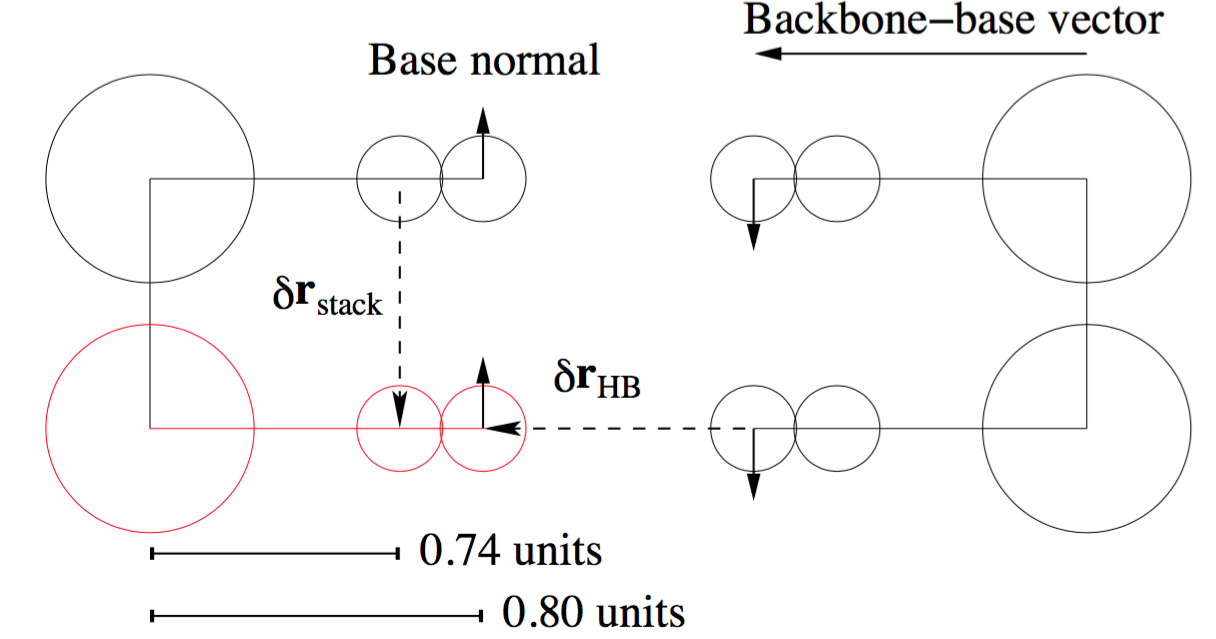
\includegraphics[width=0.7\textwidth]{./pics/model_diag-small.png}
\caption{\label{model_diag-small} Illustration of interaction sites, the backbone-base vector and base normal vector.}
\end{center}
\end{figure}


\begin{figure}[htpb]
\begin{center}
\begin{minipage}{0.4\textwidth}
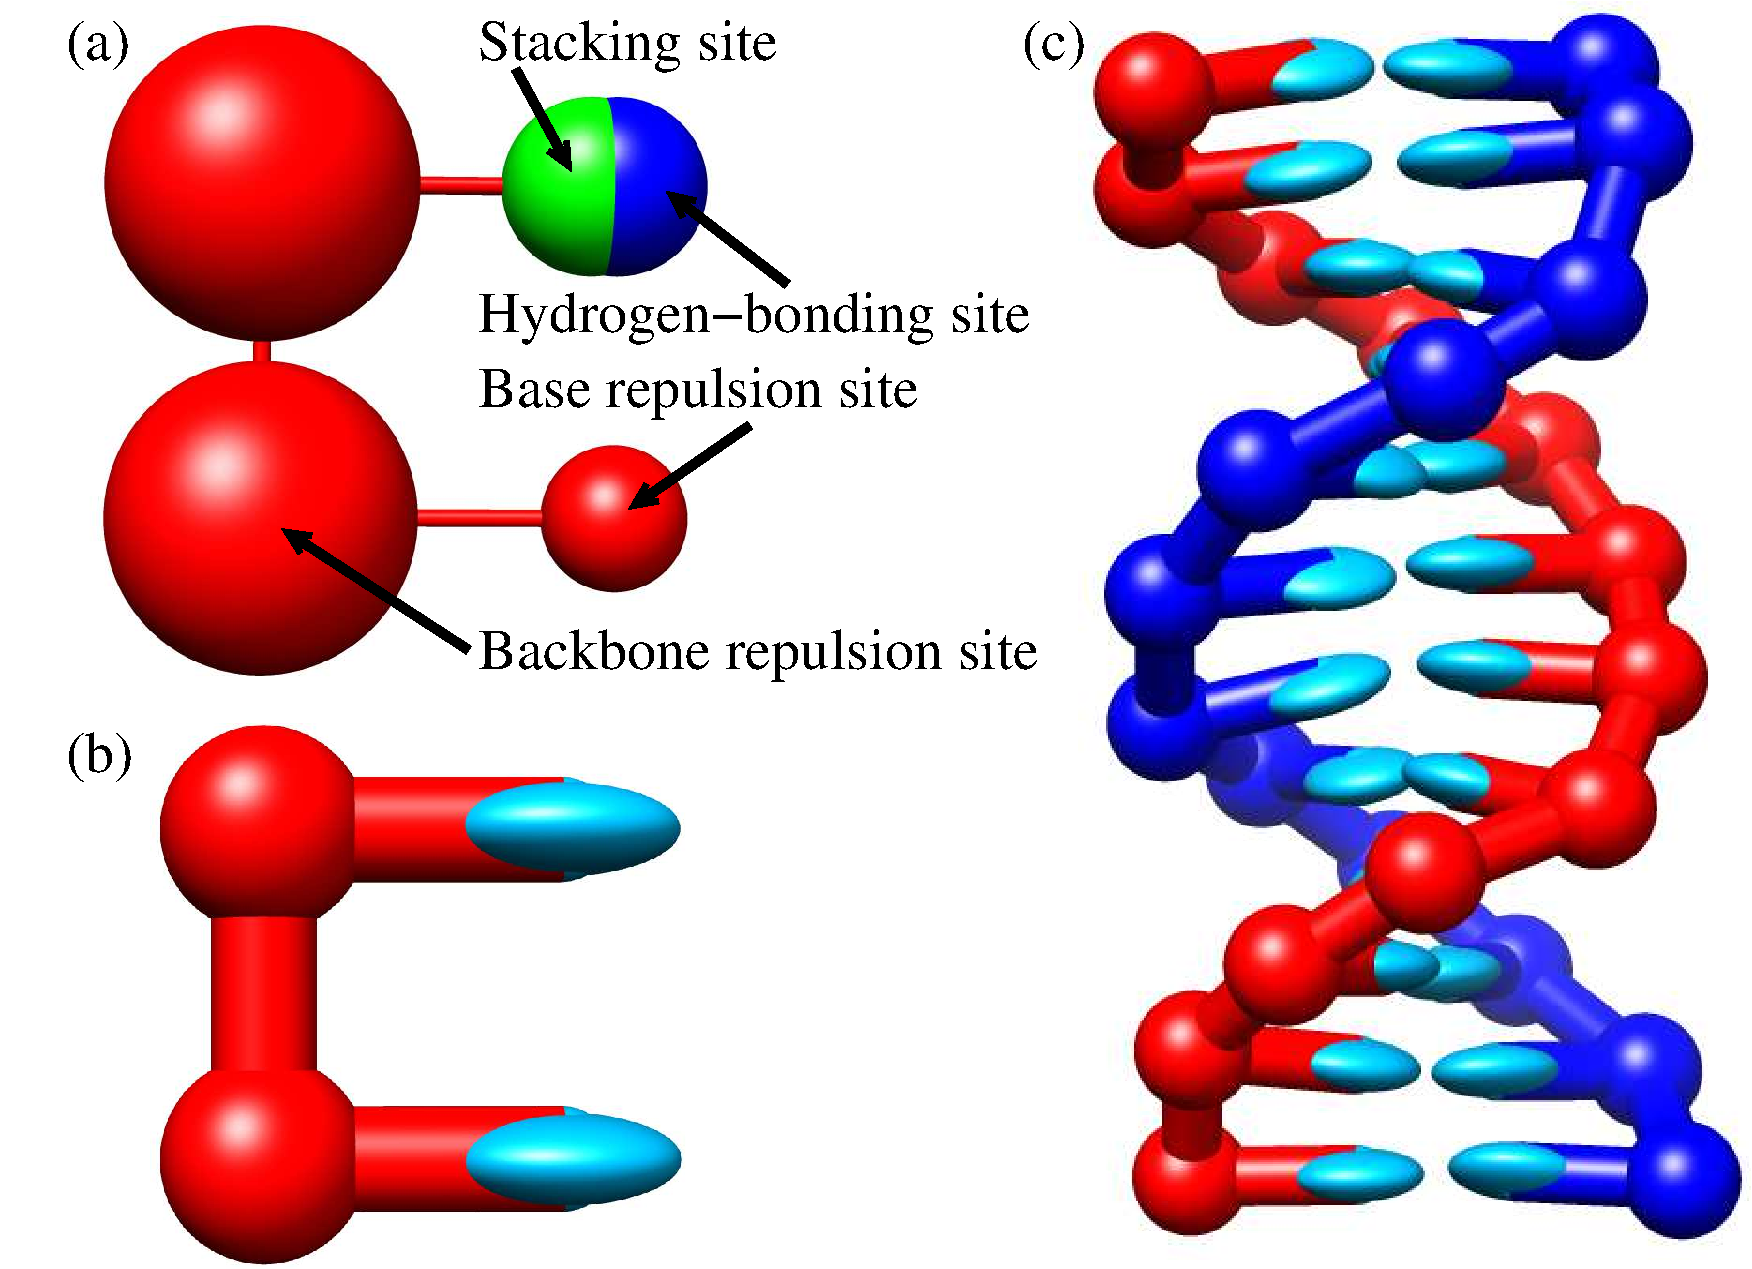
\includegraphics[width=\textwidth]{./pics/the_model-eps-converted-to.pdf}
\end{minipage}
\begin{minipage}{0.5\textwidth}
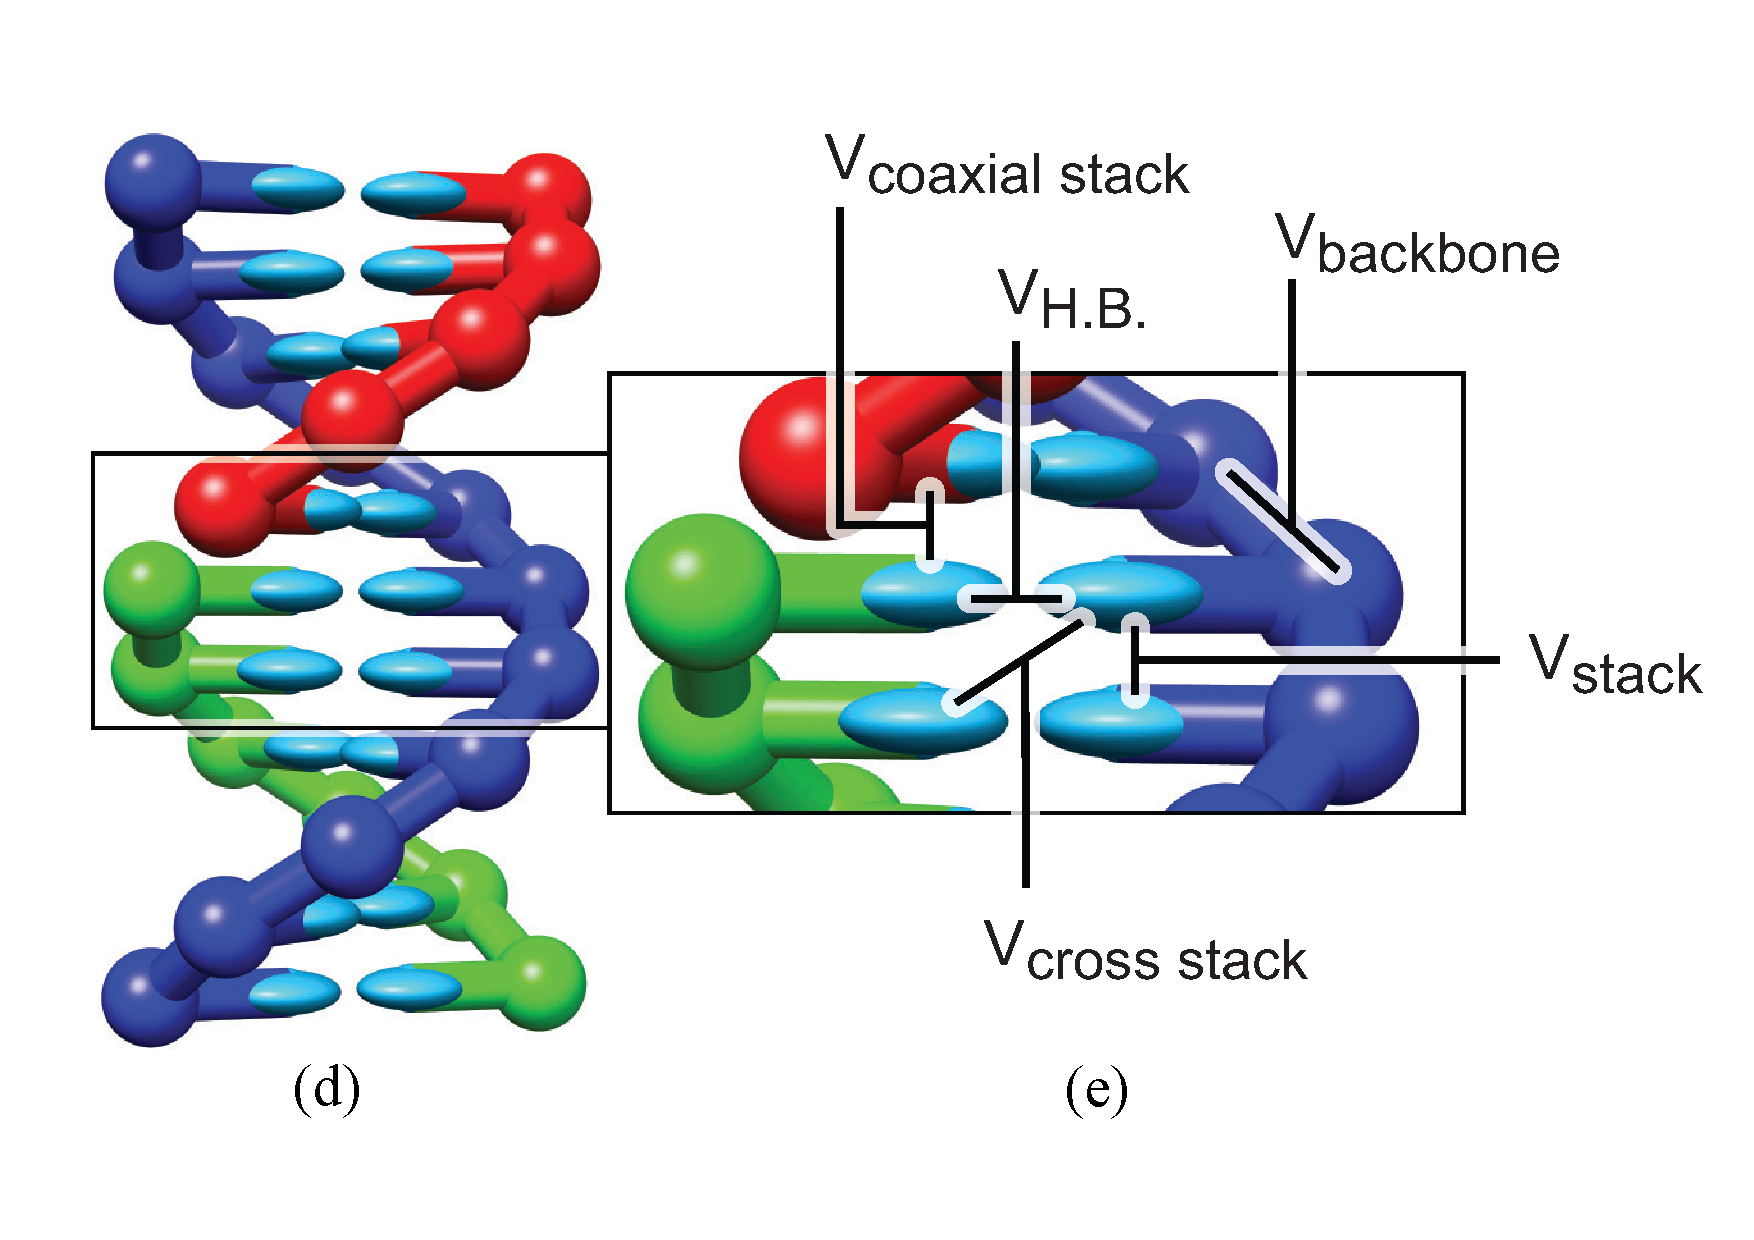
\includegraphics[width=\textwidth]{./pics/oxDNA_nicked_duplex_interactions.pdf}
\end{minipage}
\caption{\label{model} (a): Model interaction sites. For clarity, the stacking/hydrogen-bonding sites are shown on one nucleotide and the base excluded volume on the other. The sizes of the spheres correspond to interaction ranges: two repulsive sites interact with a Lennard-Jones distance unit equal to the sum of the radii shown. The distance at which hydrogen-bonding and stacking interactions are at their most negative is given by the diameter of the spheres. The subfigures (a) and (b) represent identical nucleotides on the same scale. (c): A 12 base pair duplex as represented by the model. (d): A nicked duplex with one continuous strand (blue) and two interrupted, complementary strands (red and green). (e): A close-up picture with schematic indication of the various pairwise interactions.}
\end{center}
\end{figure}

The simplest interaction is the backbone connectivity, which is modelled with FENE (finitely extensible nonlinear elastic) springs acting between the backbone interaction sites. The excluded volume interaction is modelled with truncated and smoothed Lennard-Jones potentials between backbone sites, base sites and between the backbone and base sites. 
The hydrogen bonding interaction consists of smoothed, truncated and modulated Morse potentials between the hydrogen bonding site.
The stacking interaction is formed by individual sub-interactions, namely stacking between consecutive nucleotides on the same strand, 
cross-stacking between nucleotides on opposite strands and coaxial stacking between nicked duplexes 
(double-stranded DNA with interrupted backbones, see also Fig. \ref{model} (e).) 
The stacking interactions are modelled with a combination of smoothed, truncated and modulated Morse, harmonic angle and harmonic distance potentials. 
All interactions have been parametrised to match key thermodynamic properties of ssDNA and dsDNA such as the longitudinal and torsional persistence 
length or the melting temperature of the duplex.

\section{Code Distribution and Compilation}

The software is open source and distributed under GNU General Public License (GPL). 
On ARCHER, it is available as module \texttt{module load lammps/oxdna}.
The source code is distributed
via our main repository at 
CCPForge (\url{https://ccpforge.cse.rl.ac.uk/gf}) under the project name {\it Coarse-Grained DNA Simulation (cgdna)}.
Please send a request to join the project for full access that includes permission to browse the repository and commit changes. 
Anonymous access is also provided via subversion:\\

\smallskip
\texttt{svn checkout https://ccpforge.cse.rl.ac.uk/svn/cgdna}.\\
\smallskip

\noindent To compile the code please copy all source code in \texttt{/cgdna/trunk/oxdna/src} into your LAMMPS source directory \texttt{/lammps/src}, load the LAMMPS standard packages \texttt{MOLECULE} and \texttt{ASPHERE} 
by issuing  
\texttt{make yes-molecule yes-asphere} in \texttt{/lammps/src} and 
and compile as usual. Templates for input and data files as well as a simple setup tool for straight or helical single-stranded DNA,
DNA duplexes or arrays of DNA duplexes can be found in \texttt{/cgdna/trunk/oxdna/util}.\\  

\smallskip

\noindent In the near future, we will also distribute the software as LAMMPS USER-package. This will also include an extended documentation,
which is currently being written.



\section{LAMMPS Implementation of oxDNA}
\subsection{Input File}

In the following we discuss the structure of the input file and how the newly introduced oxDNA classes are invoked.

\noindent We work with Lennard-Jones reduced units, which are invoked in LAMMPS via

\smallskip
\texttt{units lj}
\smallskip

\noindent The system is three-dimensional.

\smallskip
\texttt{dimension 3}
\smallskip

\noindent In LAMMPS, an oxDNA nucleotide is represented as a bonded-ellipsoidal hybrid particle with the associated degrees of freedom of 
bonded particles in a bead-spring polymer (backbone connectivity) and aspherical particles 
with shape (moment of inertia), quaternion (orientation) and and angular momentum.\\

\smallskip
\texttt{atom\_style hybrid bond ellipsoid}\\
\smallskip

\noindent Users are required to suppress the atom sorting algorithm as this can lead to problems in the bond topology of the DNA.\\

\smallskip
\texttt{atom\_modify sort 0 1.0}\\
\smallskip

\noindent It is important to set the skin size correctly, which controls the extent of the neighbour lists. Too large a skin size and neighbour lists
become unnecessarily long, leading to superfluous communication. Too short and partners in the pair interactions will be
lost. 

\smallskip
\texttt{neighbor 1.0 bin}\\
\smallskip

\noindent A good way to fine-tune this parameter is to run an NVE simulation with constant energy before applying Langevin integrators.
We recommend \texttt{neighbor 2.0 bin} as a safe starting point. Likewise, frequent update of the neighbour lists can lead to an undue performance degradation. This parameter should be tuned 
as well so that no dangerous builds (as reported in the standard output of LAMMPS) occur.

\smallskip
\texttt{neigh\_modify every 1 delay 0 check yes}\\
\smallskip

\noindent The initial configuration and topology is created by means of an external setup tool (see Sec. \ref{data_setup}) and read in.\\

\smallskip
\texttt{read\_data data\_file\_name}
\smallskip

\noindent All masses are set to $3.1575$ in LJ units.

\smallskip
\texttt{set atom * mass 3.1575}
\smallskip

\noindent Note that the moment of inertia is determined through the shape parameter in the data file (see below Sec. \ref{data_setup}). 
There are four types of nucleotides (A=1, C=2, G=3, T=4), which are grouped together into a group named \texttt{all} for the integration. 

\smallskip
\texttt{group all type 1 4}
\smallskip

\noindent The new oxDNA classes with its parameters are invoked as follows:

\smallskip
\texttt{bond\_style oxdna/fene\\
bond\_coeff * 2.0 0.25 0.7525\\
pair\_style hybrid/overlay oxdna/excv oxdna/stk oxdna/hbond \&\\
\hspace*{0.75cm}oxdna/xstk oxdna/coaxstk\\
pair\_coeff * * oxdna/excv   2.0 0.7 0.675 2.0 0.515 0.5 2.0 0.33 0.32\\
pair\_coeff * * oxdna/stk    seqav 0.1 6.0 0.4 0.9 0.32 0.6 1.3 0 0.8 \&\\
\hspace*{0.75cm}0.9 0 0.95 0.9 0 0.95 2.0 0.65 2.0 0.65\\
pair\_coeff * * oxdna/hbond  seqav 0.0 8.0 0.4 0.75 0.34 0.7 1.5 0 0.7\&\\
\hspace*{0.75cm}1.5 0 0.7 1.5 0 0.7 0.46 3.141592653589793 0.7 4.0 \&\\
\hspace*{0.75cm}1.5707963267948966 0.45 4.0 1.5707963267948966 0.45\\
pair\_coeff 1 4 oxdna/hbond  seqav 1.077 8.0 0.4 0.75 0.34 0.7 1.5 0 \&\\
\hspace*{0.75cm}0.7 1.5 0 0.7 1.5 0 0.7 0.46 3.141592653589793 0.7 4.0 \&\\
\hspace*{0.75cm}1.5707963267948966 0.45 4.0 1.5707963267948966 0.45\\
pair\_coeff 2 3 oxdna/hbond  seqav 1.077 8.0 0.4 0.75 0.34 0.7 1.5 0\&\\
\hspace*{0.75cm}0.7 1.5 0 0.7 1.5 0 0.7 0.46 3.141592653589793 0.7 4.0\&\\
\hspace*{0.75cm}1.5707963267948966 0.45 4.0 1.5707963267948966 0.45\\
pair\_coeff * * oxdna/xstk   47.5 0.575 0.675 0.495 0.655 2.25 \&\\
\hspace*{0.75cm}0.791592653589793 0.58 1.7 1.0 0.68 1.7 1.0 0.68 1.5 0 0.65\&\\
\hspace*{0.75cm}1.7 0.875 0.68 1.7 0.875 0.68\\
pair\_coeff * * oxdna/coaxstk 46.0 0.4 0.6 0.22 0.58 2.0 \&\\
\hspace*{0.75cm}2.541592653589793 0.65 1.3 0 0.8 0.9 0 0.95 0.9 0 0.95\&\\
\hspace*{0.75cm}2.0 -0.65 2.0 -0.65\\
}
\smallskip

Please note that according to the LAMMPS parsing rules the ampersands (\&) represent line breaks.
Visit the LAMMPS online documentation and manual for more information and for information on oxDNA2.

\subsection{Data File and Setup Tool}\label{data_setup}

The data file contains all relevant structural parameters for the simulation, i.e. details about 
the number of atoms, the topology of the molecules, the size of the simulation box, initial velocities, etc. 
The LAMMPS implementation of oxDNA follows the standard form as discussed in the LAMMPS user manual. 
We outline the relevant parts below.\\

\noindent At the beginning of the data file the total number of particles and bonds has to be given. As we are using
hybrid particles, we need to set the same number of ellipsoids. For a standard DNA duplex consisting
of 8 complementary base pairs we need 16 atoms, 16 ellipsoids and 14 bonds, 7 on each of the two single strands.
If the strands are nicked, which we don't assume here, the number of bonds would be reduced. 

\smallskip
\texttt{16 atoms\\
16 ellipsoids\\
14 bonds\\
}
\smallskip

\noindent We use four atom types to represent the four different nucleotides in DNA (A=1, C=2, G=3, T=4). 
We use only one bond type.

\smallskip
\texttt{4 atom types\\
1 bond types
}
\smallskip

\noindent The dimensions of the simulation box are defined as follows:

\smallskip
\texttt{-20.0 20.0 xlo xhi\\
-20.0 20.0 ylo yhi\\
-20.0 20.0 zlo zhi\\
}
\smallskip

\noindent Although already stated in the input file, we need to provide again the masses of the nucleotides.

\smallskip
\texttt{Masses\\
\vspace*{0.3cm}
1 3.1575\\
2 3.1575\\
3 3.1575\\
4 3.1575\\
}
\smallskip

\noindent The nucleotides are defined after the keyword \texttt{Atoms}.
Each row contains the atom-ID (1,2,3 in the example below), the atom type (1,1,4), the position (x,y,z), 
the molecule ID (all 1 in this case), an ellipsoidal flag (1) and a density (1). 

\smallskip
\texttt{Atoms\\
\vspace*{0.3cm}
1  1  0.00000e+00  0.00000e+00  0.00000e+00  1 1 1\\
2  1  1.32744e-01 -4.29128e-01  3.75061e-01  1 1 1\\
3  4  4.84608e-01 -7.08349e-01  7.50123e-01  1 1 1\\
$\vdots$
}
\smallskip

\noindent Next we set the initial velocities, all equal to 0 in the example below.
The first column contains the atom-ID (1,2,3), the following three columns the translational,
and the last three columns the angular velocity.

\smallskip
\texttt{Velocities\\
\vspace*{0.3cm}
1  0.0  0.0  0.0  0.0  0.0  0.0\\ 
2  0.0  0.0  0.0  0.0  0.0  0.0\\ 
3  0.0  0.0  0.0  0.0  0.0  0.0\\
$\vdots$
}
\smallskip

\noindent Note that this is our special choice in the setup tool. The velocities can be generally initialised to any value.
Large values will lead to the FENE springs becoming overstretched and may provoke an early abortion of the run. 

\noindent The ellipsoids are defined with atom-ID, shape (1.17398 to produce the correct moment of inertia) 
and initial quaternion (last four columns). 

\smallskip
\texttt{Ellipsoids\\
\vspace*{0.3cm}
1   1.17398 1.17398 1.17398  1.00000e+00  0.0e+00  0.0e+00  0.00000e+00\\
2   1.17398 1.17398 1.17398  9.55336e-01  0.0e+00  0.0e+00  2.95520e-01\\
3   1.17398 1.17398 1.17398  8.25335e-01  0.0e+00  0.0e+00  5.64642e-01\\
$\vdots$
}
\smallskip

\noindent Finally, we specify the bond topology. The first column contains the bond-ID (1,2,3),
the second one the bond type (1) and the third and fourth the IDs of the two bond partners.

\smallskip
\texttt{Bonds\\
\vspace*{0.3cm}
1       1       1       2\\
2       1       2       3\\
3       1       3       4\\
$\vdots$
}
\smallskip

\noindent To simplify the setup process we created a small python tool, which can be found
in \newline \texttt{/cgdna/trunk/oxdna/util}. The syntax is

\smallskip
\texttt{python generate\_simple.py sequence.txt data\_file\_name}. 
\smallskip

\noindent The system size has to be specified directly in \texttt{generate\_simple.py}. 
The rise (separation of consecutive nucleotides) in z-direction is currently set to 
$r_0=0.7$ and should not be changed.
The output is directly written into a data file \texttt{data\_file\_name} and its name has to be stated in 
the LAMMPS input file. \texttt{sequence.txt} is an ASCII input file that contains 
keywords and the sequence on one ssDNA strand. Several options are available:

\smallskip
\texttt{single 0,0,0:ACGTA} 
\smallskip

\noindent creates a single straight DNA strand (with five adenine nucleotides in the above example). 
The first nucleotide is
positioned at $(x,y,z)=(0,0,0)$. The four remaining nucleotides are then added in positive
z-direction with a rise of $r_0=0.7$. 

\smallskip
\texttt{single\_helix 0,0,0:ACGTA}
\smallskip

\noindent produces a helically twisted single strand similar to the above one, but with a twist angle of $0.6$
radian between consecutive nucleotides. This twist angle is set in the script and should not be altered as it leads to a reasonably 
stable configuration that can be further equilibrated.

\smallskip
 \texttt{duplex 0,0,0:ACGTA}
\smallskip

\noindent creates a DNA duplex. This is done by forming a helically twisted single strand with the sequence stated
in \texttt{sequence.txt}, which is then complemented by the corresponding bases on a second, helically twisted 
strand to form complete base pairs, in the above case \texttt{TGCAT}.
 
\smallskip
\texttt{duplex\_array 10,10:-20:ACGTA}
\smallskip

\noindent produces an array of duplexes oriented along the z-direction. 
In the above example the array consists of $10 \times 10$ duplexes with five base pairs each.
The first nucleotide on the first strand of the first duplex is positioned at $z=-20$. The duplexes
are equally distributed in the x- and y-direction.  

\section{Langevin-Type Rigid-Body Integrators}

We also implemented novel Langevin-type rigid-body integrators that were developed
by Davidchack, Ouldridge and Tretyakov (see Ref. \cite{Davidchack:2015}).
The motivation for this was that previously no really good Langevin integrators for rigid bodies
existed in LAMMPS.
Without noise all integrators A, B and C in the above reference are identical.
We refer to this case as the ``DOT integrator''. This is an alternative to the  
standard LAMMPS NVE integrator for aspherical particles, and can be invoked by replacing

\smallskip
\texttt{fix 1 all nve/asphere}\\
\smallskip

\noindent with

\smallskip
\texttt{fix 1 all nve/dot}\\
\smallskip

\noindent in the input file. This energy-conserving integrator is useful to study the accuracy of the 
integrator or the integrity of the pair interactions at a given timestep size $\Delta t$.

\noindent The C integrator in Ref. \cite{Davidchack:2015}, to which we refer as ``DOT-C integrator'',
 is invoked by replacing the standard NVE integrator 
for aspherical particles and the fix for Langevin dynamics 

\smallskip
\texttt{fix 1 all nve/asphere}\\
\texttt{fix 2 all langevin 0.1 0.1 0.03 457145 angmom 10}\\
\smallskip

\noindent with a single fix

\smallskip
\texttt{fix 1 all nve/dotc/langevin 0.1 0.1 0.03 457145 angmom 10}.\\
\smallskip


\begin{figure}[htpb]
\begin{center}
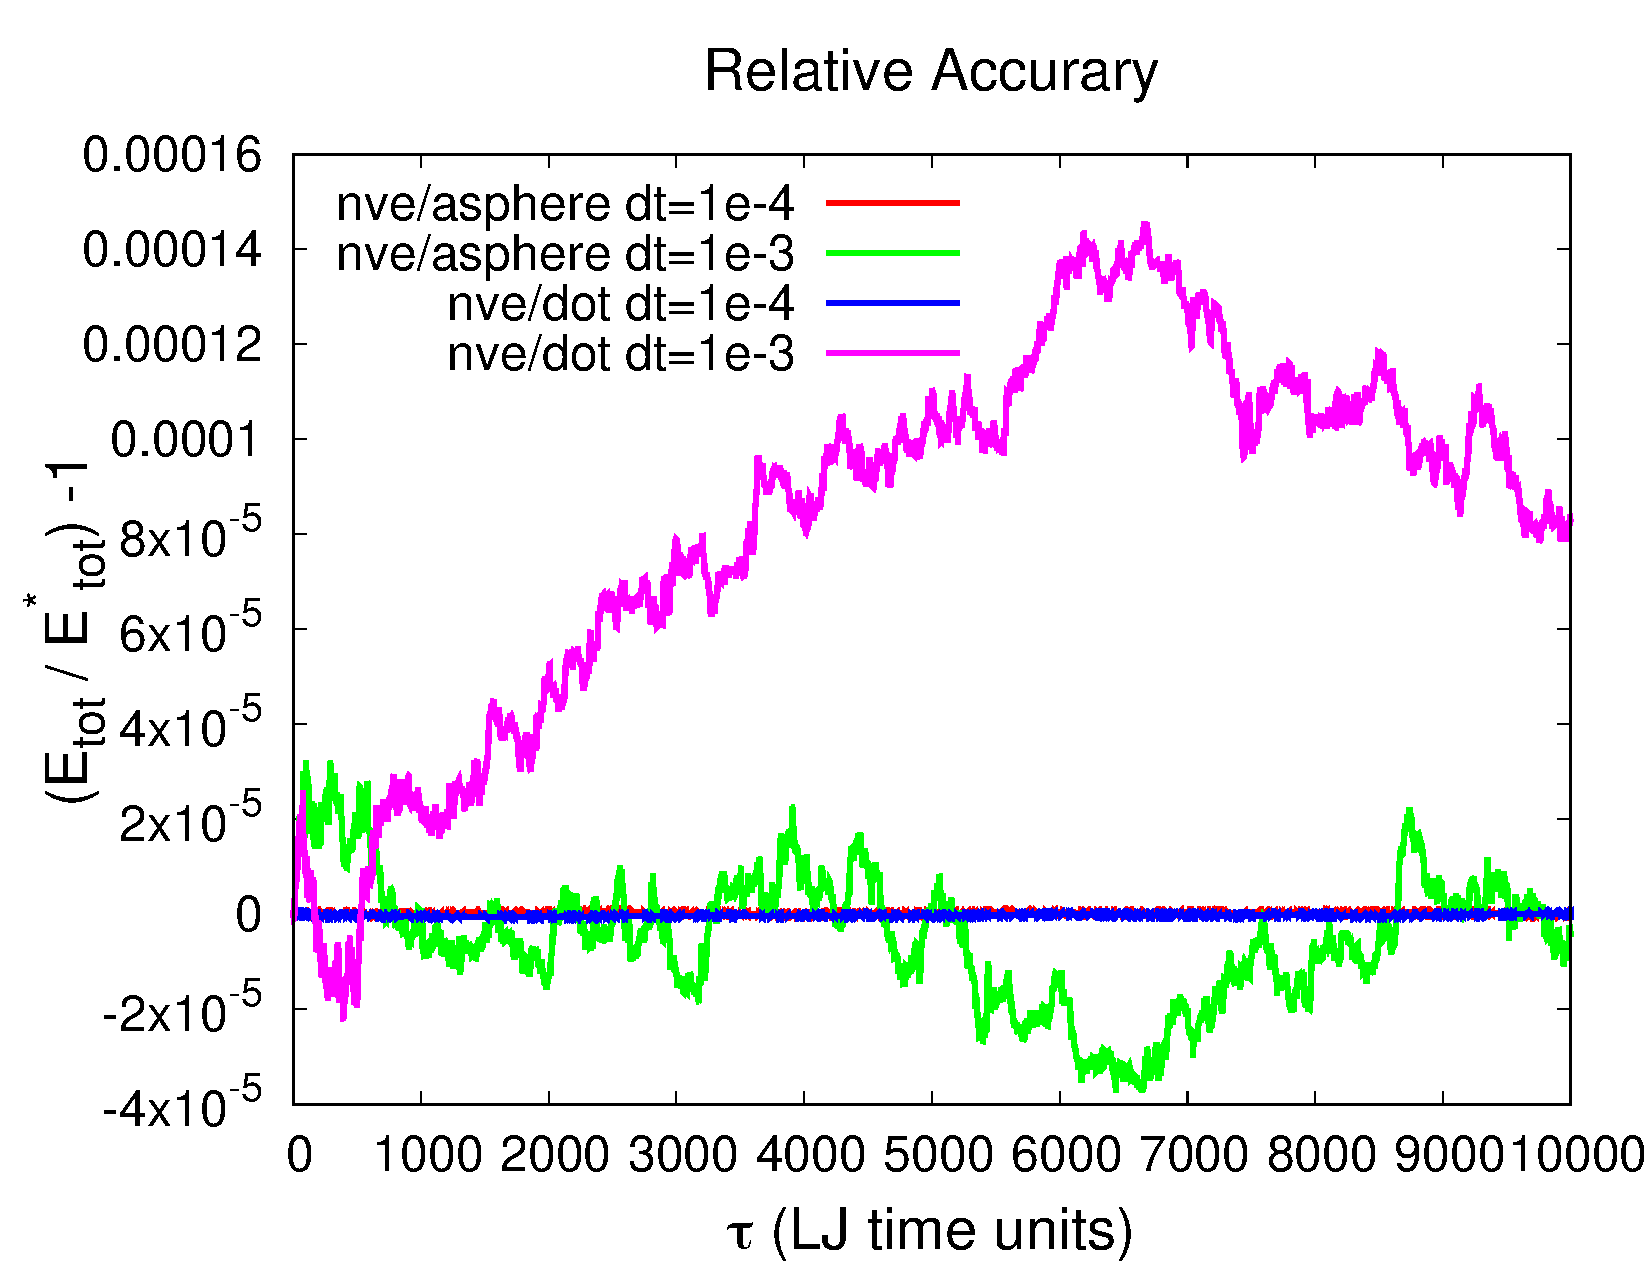
\includegraphics[width=0.8\textwidth]{./pics/etot_nve_asphere_dot.pdf}
\caption{\label{integrator} Relative normalised accuracy $(E_{tot}-E^*_{tot})/E^*_{tot}$ of the standard LAMMPS NVE integrator 
for aspherical particles and the NVE DOT integrator from Ref. \cite{Davidchack:2015}. $E^*_{tot}$ is the total free energy 
at the beginning of the simulation runs.}
\end{center}
\end{figure}

\noindent To measure the accuracy of the new integrators we run a test case consisting of a short, 
nicked duplex with 8 base pairs (16 nucleotides). 
Fig. \ref{integrator} shows the accuracy measured through the normalised difference between the total energy $E_{tot}$ for
this particular benchmark and the total energy at the beginning of the run $E_{tot}^*$. 
We compared the standard \texttt{fix nve/asphere} integrator, 
which is based on a Richardson iteration in the update of the quaternion degrees of freedom, to the new DOT integrator, 
which uses a rotation sequence to update the quaternions. Shown are results for two different timestep sizes
$\Delta t=10^{-3}$ and $\Delta t=10^{-4}$. Both simulations were run for the same physical simulation time to allow
 direct comparison of the deviations of a dynamical run. As this is done in the NVE ensemble and without noise, 
the energy should be exactly conserved. This corresponds to a straight, horizontal line at 0.

It is obvious that above a certain timestep size the accuracy of the new DOT integrator is slightly 
inferior compared to the standard integrator. Up to a certain point the DOT integrator actually seems to deviate 
further from the correct result, whereas the standard integrator oscillates more around the correct value. 
This, however, is more or less a transient effect as longer runs show there is no permanent drift away from the correct
result. 

\begin{table*}[htpb]
\begin{center}
\begin{tabular}{ | c | c | c | c | c | c | c |}
\hline
& $\Delta t$ & $E_{kin}$ & $E_{rot}$ & $E_{pot}$ & $E_{tot}$ & standard error of $E_{tot}$ fit\\
\hline
\hline
fix nve/asphere \& & & & & & &\\
fix langevin & & & & & &\\
\hline
& $10^{-4}$ &2.3999 &2.4001  &-21.4512 &-16.6513 & $\pm$ 0.00377  (0.0227\%)\\
\hline
& $10^{-3}$ & 2.4015  &2.4021  &-21.5564 &-16.7582 & $\pm$ 0.00349 (0.0208\%)\\
\hline
& $5\cdot10^{-3}$ &2.4012  &2.3999  &-21.6352  &-16.8315  & $\pm$ 0.00322 (0.0191\%)  \\
\hline
\hline
nve/dotc/langevin & & & & &\\
\hline
& $10^{-4}$ &2.3989 &2.3997 &-21.5278 &-16.7292 & $\pm$ 0.00362 (0.0216\%)\\
\hline
& $10^{-3}$ &2.3998 &2.4008 &-21.6631 &-16.8624 & $\pm$ 0.00335 (0.0199\%)\\
\hline
& $10^{-2}$ & 2.3959 & 2.3941  &-21.6151 &-16.8251 & $\pm$ 0.00318 (0.0189\%) \\
\hline
& $2\cdot10^{-2}$ &2.3895  & 2.3752 &-21.6266   &-16.8619  & $\pm$ 0.00313 (0.0185\%)\\
\hline
\end{tabular}
\end{center}
\caption{\label{table1} Average kinetic, rotational, potential and total energy for the standard LAMMPS integrator \texttt{fix nve/asphere} \&
\texttt{fix langevin} and the DOT-C integrator \texttt{nve/dotc/langevin} for different timestep sizes.}
\end{table*}   

For Langevin dynamics, it is not possible to evaluate the accuracy and stability in the same way.
We opted instead for an estimate based on the average kinetic, rotational, potential and
total energy of the benchmark. Again, we performed runs of $\tau=10000$ Lennard-Jones time units length, this time thermalised, 
and fitted the results with a standard least-square procedure. The number of MD-timesteps and the output frequency for each timestep size 
were adapted so that the total physical simulation time and the statistical basis of the error calculations were consistent. 
The temperature in reduced LJ-units was set to $T=0.1$, whereas the translational and rotational friction coefficients 
were set to $\gamma=1/0.03$ and $\Gamma=1/0.3$, respectively.
The results are summarised in Tab. \ref{table1}.

Based on three translational and three rotational degrees of freedom per nucleotide and 8 base pairs we expect kinetic and rotational energies $E_{kin}=E_{rot}=2.4$ 
for a temperature settings $T=0.1$. This is very well achieved for all timestep sizes and both integrators, the standard LAMMPS integrator \texttt{fix nve/asphere \& fix langevin} and the DOT-C integrator \texttt{fix nve/dotc/langevin}, whereas there appears to be a slight decrease in the 
DOT-C integrator for very large step sizes ($\Delta t=2\cdot10^{-2}$).
The deviation of the total energy between all timestep sizes, admittedly a {\it ad hoc} criterium to quantify the stability of the integrators,
but one that is rather hard for the integrators to get exactly right, is in the sub-percent range.
It is actually slightly better for the DOT-C integrator than for the standard LAMMPS integrator. 
The statistical errors, reported in Tab.\ref{table1}, are the standard deviations of a linear least square fit and 
show that the deviations are well above the uncertainty of the fits.

Remarkably, for the DOT-C integrator the limit for a stable integration is $\Delta t=2\cdot10^{-2}$, which represents a very large timestep size. 
This is about 4 times larger than the maximum timestep size for which the standard LAMMPS Langevin integrator produces sound results.
Because of the more complex rotations in quaternion space and various additional transformations that the DOT-C integrator requires
there is a small overhead of about $15\%$ compared to the standard LAMMPS integrator. Nevertheless, this small overhead of the DOT-C
integrator is very well compensated by the computational efficiency and possibility to increase the timestep 
size by $400\%$ (from a maximum of $\Delta t=5\cdot10^{-3}$ for the standard LAMMPS integrator to $\Delta t=2\cdot10^{-2}$ for the DOT-C integrator).


\section{Performance Analysis}

We devised a few simple benchmarks to study the parallel performance of the LAMMPS implementation. The size of each benchmark is well beyond the 
current capabilities of the standalone version, so demonstrates as well a minimal performance requirement. 
The benchmarks consisted of arrays of double-stranded, regularly arranged DNA duplexes, each with a length of 600 base pairs.
The low-density (LD) benchmark was formed by an array of $10 \times 10$ duplexes, giving a total of 60 kbp, and is shown in Fig. \ref{bench-60kbps}. 
The high-density (HD) benchmark was formed by an array of $40\times 40$ duplexes with a density 16 times larger than the LD case and a total number
of 960 kbp.

\begin{figure}[htpb]
\begin{center}
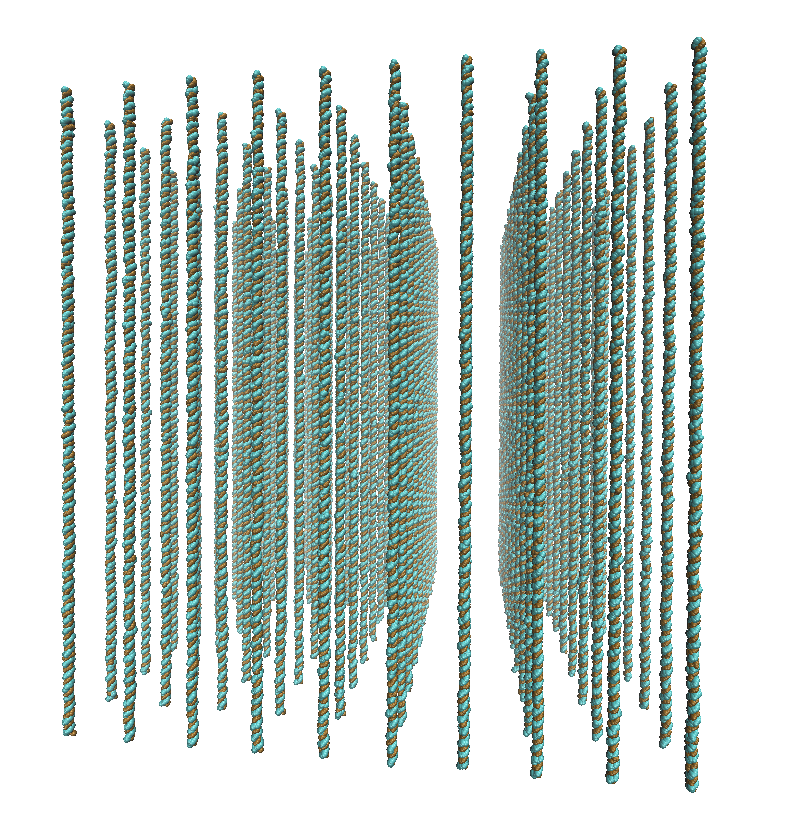
\includegraphics[width=0.4\textwidth]{./pics/bench_60kbps.png}
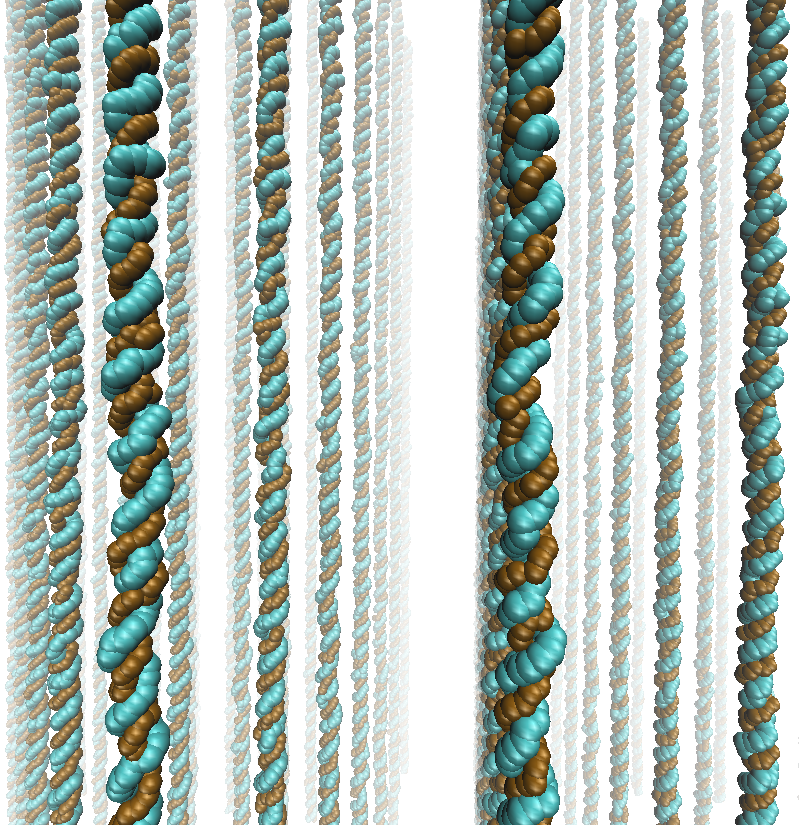
\includegraphics[width=0.4\textwidth]{./pics/bench2_60kbps.png}
\caption{\label{bench-60kbps} The low-density benchmark consisting of an array of $10\times 10$ DNA duplexes with a length of 600 base pairs each, in total 60 kbp. The high-density benchmark (not shown) consisted of a similar array of $40\times 40$ duplexes with 960 kbp in total.}
\end{center}
\end{figure}

\begin{figure}[htpb]
\begin{center}
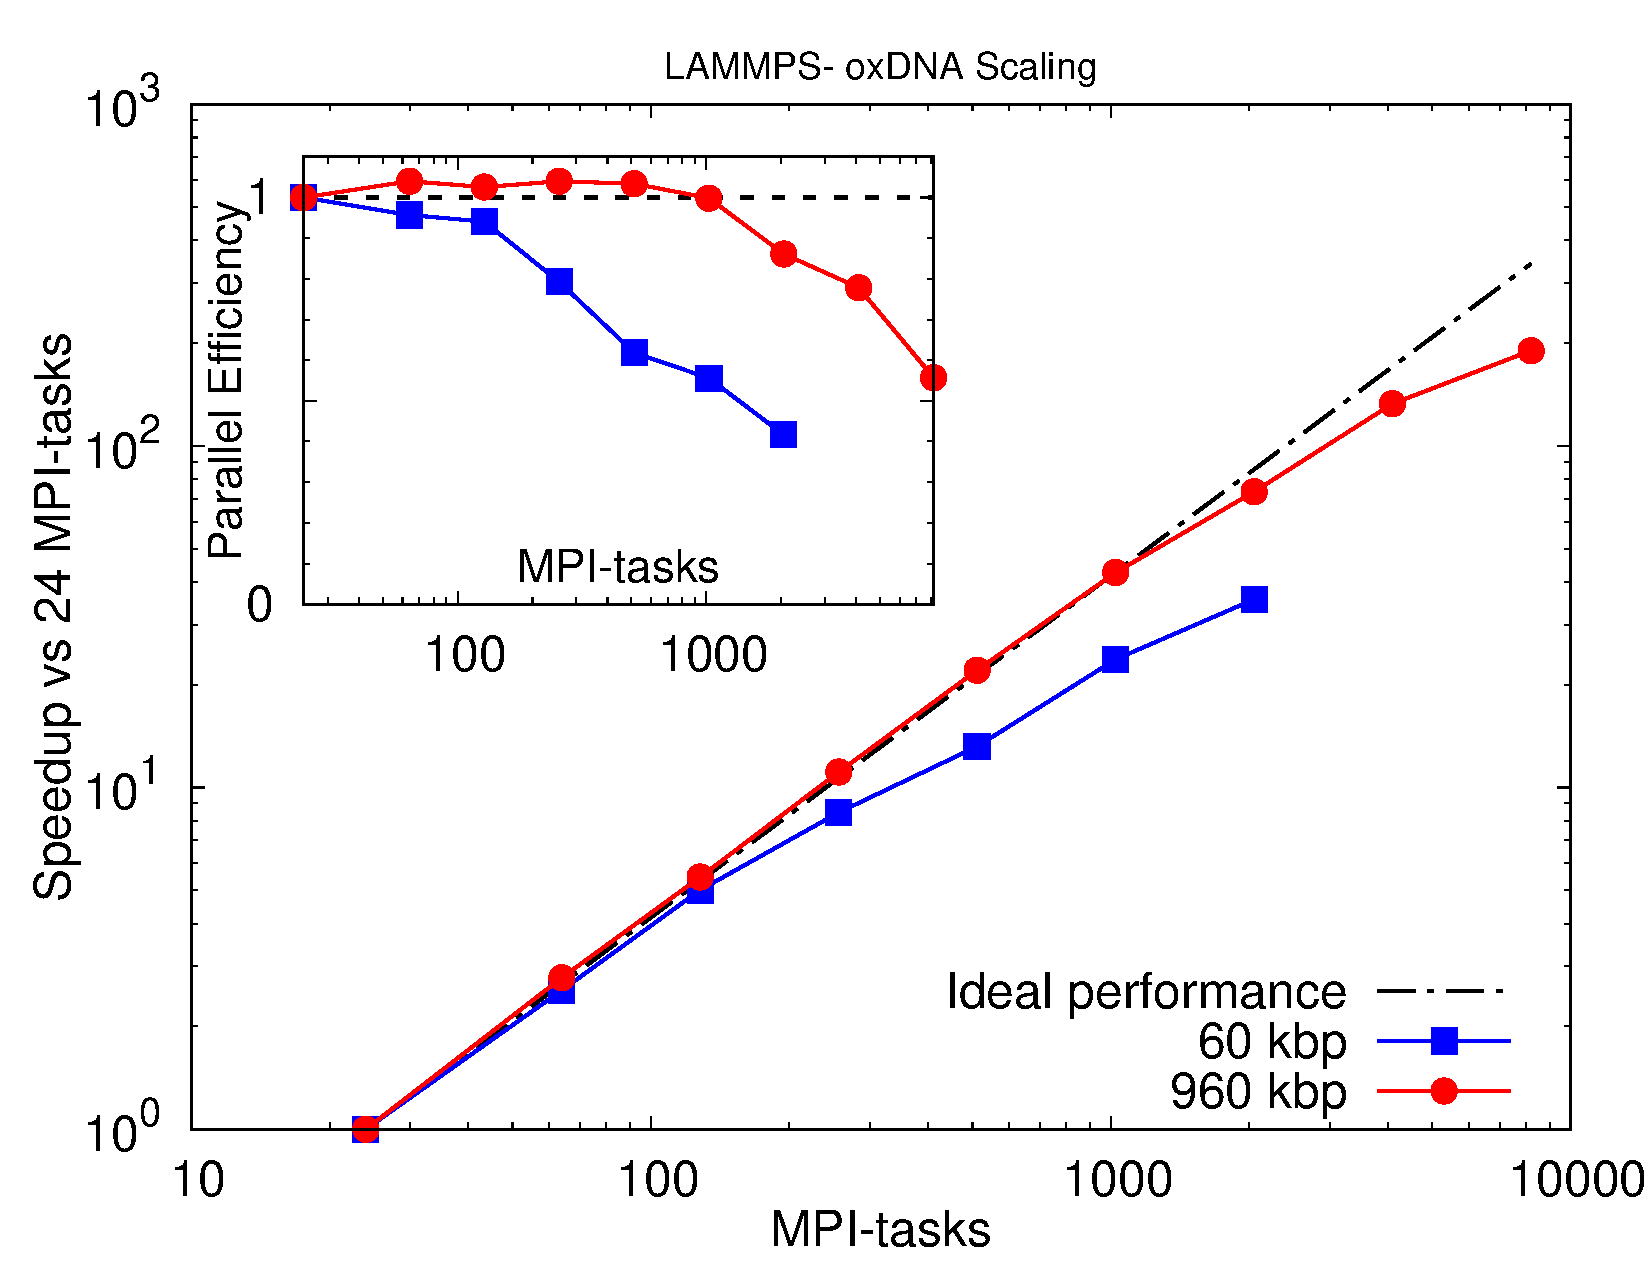
\includegraphics[width=0.7\textwidth]{./pics/LAMMPS_oxdna_scaling.pdf}
\caption{\label{scaling} Strong scaling behaviour: Speedup of the low and high density benchmarks of 60 kbp and 960 kbp, respectively, compared
to the single node performance with 24 MPI-tasks. The inset shows the parallel efficiency relative to the single node case with 24 MPI-tasks.}
\end{center}
\end{figure}

Whilst a regular array of double-stranded DNA strands appears perhaps somewhat artificial, it creates a reasonably load-balanced 
situation and facilitates the performance analysis. The obtained densities of DNA, are however very well comparable to 
those of DNA gels \cite{Rovigatti:2014} and high density states of DNA which form liquid-crystalline phases \cite{DeMichele:2012}.

Strong scaling tests were performed on ARCHER on up to 86 nodes (LD) and 342 nodes (HD), respectively.
The benchmark cases were run for 30,000 (LD) and 10,000 (HD) MD-timesteps with a timestep size of $\Delta t=5\times10^{-3}$.
We used the standard LAMMPS integrators for Langevin dynamics, i.e. the \texttt{fix nve/asphere} and \texttt{fix langevin}.
The primary reason for this was that the wallclock time for runs with the standard integrator was still a few
percent shorter, although the improved efficiency of the DOT-C integrator would mean these runs were shorter in physical time. 
The temperature in reduced LJ-units was $T=0.1$, whereas the translational and rotational friction coefficients were set to 
$\gamma=1/0.03$ and $\Gamma=1/0.3$, respectively.

Fig. \ref{scaling} shows the parallel speedup for both benchmarks relative to the single node performance with 24 MPI-tasks. The code performs well
for the LD benchmark up to about 128 MPI-tasks with a parallel efficiency around $95\%$ (see the inset). Beyond several hundred MPI-tasks a gradual performance 
degradation is observed. At 2048 MPI-tasks the parallel efficiency has decreased to about $40\%$ and the total speedup is roughly 
850 compared to the single core performance (35 compared to the single node performance). 


A look at the ratio of the number of local atoms to the number of ghost atoms on each process 
proves that this performance degradation is due to the size of the problem. At the largest core counts 
there are on average only about 60 local atoms present on each process. The number of ghost atoms is at the same time in the range of 225 atoms, 
so almost four times as large. LAMMPS is known to require at least a few hundred local atoms or more for a good parallel performance \cite{LAMMPSdoc}. 
The reason why the speedup is still relatively good lies in the fraction of time that the algorithm spends in the force calculation,
which is still comparably large.

For the HD benchmark, 16 times larger than the LD case, the performance degradation is almost exactly mirrored at core counts which are 
about 16 times larger. For the HD benchmark the total speedup at 8192 MPI-tasks is just below 4600 with respect to the single core performance 
(190 compared to the single node performance) and the parallel efficiency is still above $50\%$.


\section{Profiling}

We used the Craypat Performance Tools on ARCHER to conduct sampling experiments of the benchmarks. Fig. \ref{perf-60kbps} shows a pie chart
of the low density (LD) run. The image on the left shows the results on a single node with 24 MPI-tasks, whereas the image on the right 
is for 2048 MPI-tasks.
Focussing first on a single node, calls to the MPI-library are below $5\%$ and do not appear with an individual pie section. 
The total time spent in the force calculation is around $86\%$ (according to the LAMMPS breakdown).
Interestingly, a significant fraction of the time is spent on calculating the local body coordinate system of the nucleotide from the quaternion 
degrees of freedom (MathExtra::q\_to\_exy, $11.3\%$).

\begin{figure}[htbp]
\centering
\begin{minipage}{0.92\textwidth}
\centering
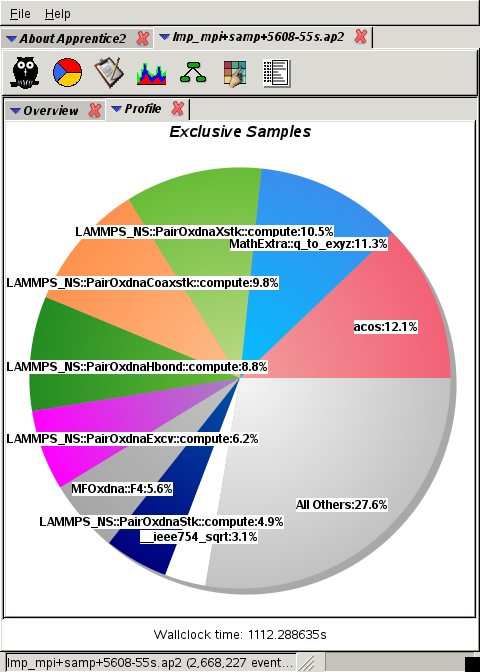
\includegraphics[width=0.44\textwidth]{./pics/n1_opt_screenshot1_60kbps.png}
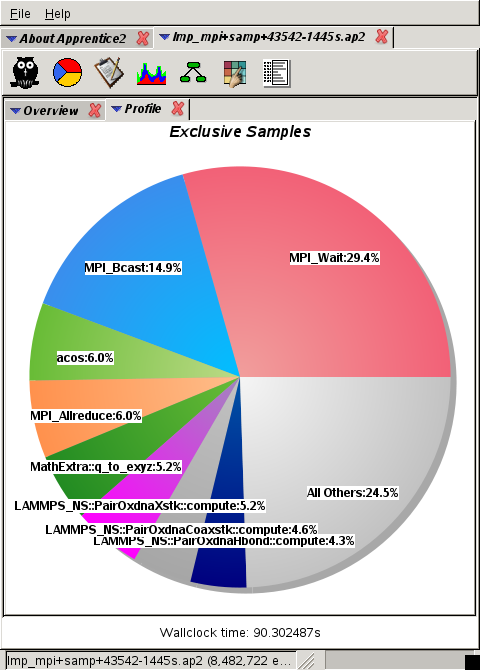
\includegraphics[width=0.443\textwidth]{./pics/p2048_opt_screenshot1_60kbps.png}
\caption{\label{perf-60kbps} Craypat performance analysis of a sampling experiment for the low density benchmark (60 kbp) on a single node (left, 24 MPI-tasks) and for 2048 MPI-tasks (right). Note that the assigned colour code for the functions is different in both cases.}
\end{minipage}
\end{figure}
\begin{figure}[htbp]
\centering
\begin{minipage}{0.92\textwidth}
\centering
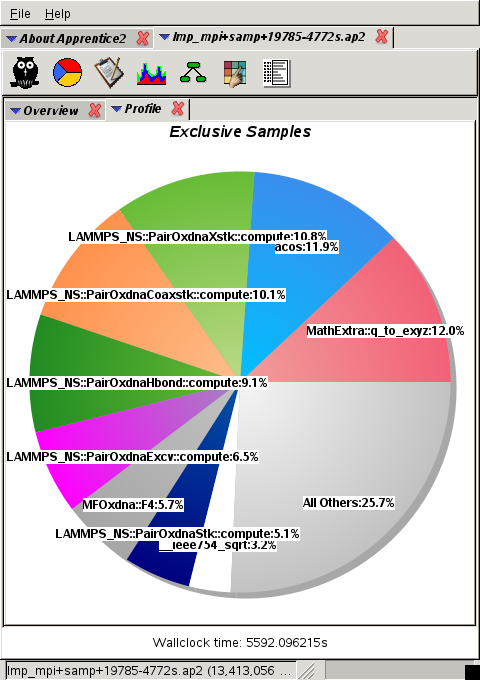
\includegraphics[width=0.43\textwidth]{./pics/n1_opt_screenshot1_1mbps.png}
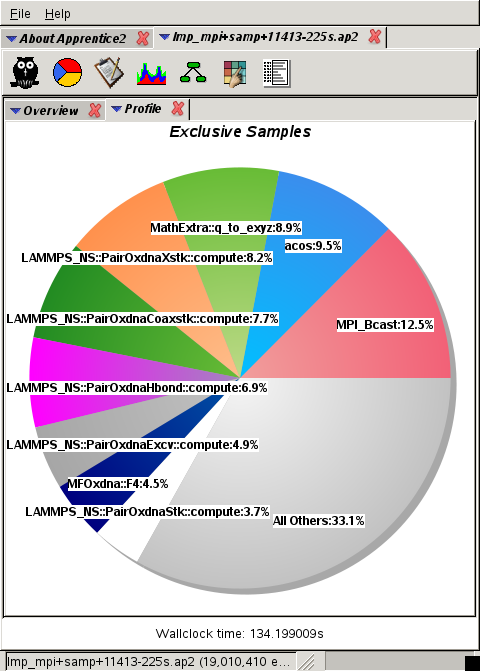
\includegraphics[width=0.437\textwidth]{./pics/p2048_opt_screenshot1_1mbps.png}
\caption{\label{perf-1mbps}Craypat performance analysis of a sampling experiment for the high density benchmark (960 kbp) on a single node (left, 24 MPI-tasks) and for 2048 MPI-tasks (right). Note that the assigned colour code for the functions is different in both cases.}
\end{minipage}
\end{figure}

A significant portion falls also on the calculation of the inverse cosine (acos, $12.1\%$). 
The conversion from quaternions to 3-vectors is done separately in every single interaction. 
This has been done for simplicity, but represents a 6-fold overhead as it could be optimised by calculating the 3-vectors only once per timestep,
then saving the for later use by the interactions. This optimisation would come at increased communication as the additional nine
components of the three unit vectors would have to be communicated across the process boundaries.
Another possibility, and a major adaptation, would be to formulate the entire force calculation in generalised quaternion forces and torques, 
therefore avoiding the transformation in the first place. We decided deliberately against this possibility as this would require 
calculation of four force and torque components in quaternion space. The calculation with 3-vectors on the other hand, as currently implemented, 
requires only three force and torque components. They can also be fed directly to the other LAMMPS routines. It is thus very likely 
that a performance gain from avoiding the transformation would be outweighed by the larger number of additional components and generalised
quaternion forces and torques which also had to be communicated across the process boundaries.

The large fraction of the inverse cosine is more difficult to optimise. It emerges in the stacking, cross- and coaxial stacking
and hydrogen bonding interactions through a partial derivative with respect to the relative distances. A previous version of the 
implementation spent a whopping $29\%$ of its time calculating the inverse cosine. This prohibitively large figure could be 
cut down to the current $12 \%$ by introducing appropriate early-rejection criteria in each force calculation. Further improvements
might be possible through small-argument approximations of the inverse cosine. This will be tested in a future version
of the code (e.g. for the upgrade to oxDNA 2.0).

At 2048 MPI-tasks, shown on the right of Fig. \ref{perf-60kbps}, the code spends more than $50\%$ of its time in call to the MPI-library.
The percentage of time in the force calculation has fallen to about $43\%$. As stated above, this is primarily the consequence of 
an insufficient number of local atoms with respect to the number of ghost atoms, and does not reflect a problem with the 
parallel performance of the implementation.  

For the HD benchmark on a single node, shown on the left in Fig. \ref{perf-1mbps}, calls to the MPI-library are below $3\%$.
The conversion of quaternions to 3-vectors (MathExtra::q\_to\_exyz) and the calculation of the inverse cosine (acos) are constant 
at about $12\%$. At 2048 MPI-tasks we observe a parallel efficiency of about $85\%$. The time spent in the force calculation is
still about $82\%$ (according to the LAMMPS breakdown) with calls to the MPI-library amounting to just below $13\%$. 
The CPU time of the quaternion conversion to the local body frame of the nucleotide and the inverse cosine each at are around $9\%$ 
due to the larger share of the calls to the MPI-library.

%\clearpage

\section{Conclusions}

We developed an implementation of the oxDNA model for coarse-grained DNA simulation which is based on the LAMMPS code. 
The results of the scaling tests and performance analysis are very encouraging and demonstrate that LAMMPS is absolutely  
capable of tackling large and extremely large problems, which are well beyond what could be reached by the standalone version. 
It is worth mentioning that the GPU-accelerated version of the standalone code can only achieve speedups of up to a 
factor 30 compared to the single core performance. The scaling analysis of the benchmarks gives evidence 
that this is can be easily matched on a single ARCHER node with 24 MPI-tasks and an MPI-only implementation.

The newly implemented Langevin-type rigid-body integrators, particularly the DOT-C integrator, offer an additional advantage
over the existing standard LAMMPS rigid-body integrators for Langevin dynamics. At the costs of a small additional overhead 
they allow considerably larger timesteps and show improved stability.

We consider this project also as a starting point for multiscale modelling of DNA. This could be achieved through combining 
different CG and atomistic models in one single simulation. Through its extendibility and 
excellent performance LAMMPS appears ideally suited for such an undertaking.

\bibliographystyle{unsrt}
\bibliography{eCSE05-10_Technical_Report} %your .bib file

\end{document}
